% This is samplepaper.tex, a sample chapter demonstrating the
% LLNCS macro package for Springer Computer Science proceedings;
% Version 2.20 of 2017/10/04
%
\documentclass[runningheads]{llncs}
%
\usepackage{graphicx}
\usepackage[portuges]{babel}
\usepackage[utf8]{inputenc}
\usepackage[T1]{fontenc}
\usepackage{verbatim}
\usepackage{float}
\usepackage{caption}
\usepackage{subfig}
\usepackage[hidelinks]{hyperref}
%Path relative to the .tex file containing the \includegraphics command
\graphicspath{ {./images/} }
% Used for displaying a sample figure. If possible, figure files should
% be included in EPS format.
%
% If you use the hyperref package, please uncomment the following line
% to display URLs in blue roman font according to Springer's eBook style:
% \renewcommand\UrlFont{\color{blue}\rmfamily}
\setcounter{secnumdepth}{6}
\renewcommand\theparagraph{\Alph{paragraph}}
 
\makeatletter
\renewcommand\paragraph{\@startsection{paragraph}{4}{\z@}%
                                      {-3.25ex\@plus -1ex \@minus -.2ex}%
                                      {0.0001pt \@plus .2ex}%
                                      {\normalfont\normalsize\bfseries}}
\renewcommand\subparagraph{\@startsection{subparagraph}{5}{\z@}%
                                      {-3.25ex\@plus -1ex \@minus -.2ex}%
                                      {0.0001pt \@plus .2ex}%
                                      {\normalfont\normalsize\bfseries}}
 
\counterwithin{paragraph}{subsubsection}
\counterwithin{subparagraph}{paragraph}
\makeatother
\hyphenation{ProcessID}
\newlength{\common}
\begin{document}
%
\title{Melhoria Bases de dados NoSQL}
%
\titlerunning{Bases de dados NoSQL}
% If the paper title is too long for the running head, you can set
% an abbreviated paper title here
%
\author{ Henrique José Carvalho Faria nº82200 }
%
% First names are abbreviated in the running head.
% If there are more than two authors, 'et al.' is used.
%
\institute{Departamento de Informática, Universidade do Minho}
%
\maketitle              % typeset the header of the contribution
%
% Abstract
\begin{abstract}


Neste trabalho foi pedido que se criasse uma base de dados em MySQL e que se povoasse a mesma com 3 clubes, tendo cada clube 1 treinador e 11 jogadores. Posteriormente escolheu-se implementar a mesma base de dados utilizando o mongoDB e construiu-se um modelo de dados capaz de dar resposta a uma aplicação que a utilize. Por fim, enunciaram-se as diferenças entre uma base de dados relacional e a base de dados escolhida.


\keywords{MySQL \and MongoDB}
\end{abstract}
%
%

\newpage
\newpage
\hfill
% Aqui começam os capitulos abordados pelo trabalho
\section{Questão 1}

A base de dados apresentada foi recriada recorrendo á aplicação MySQLWorkbench\cite{ref_intro} e foi povoada utilizando o seguinte script:

\begin{figure}[H]

  \centering
  \captionsetup{justification=centering}

  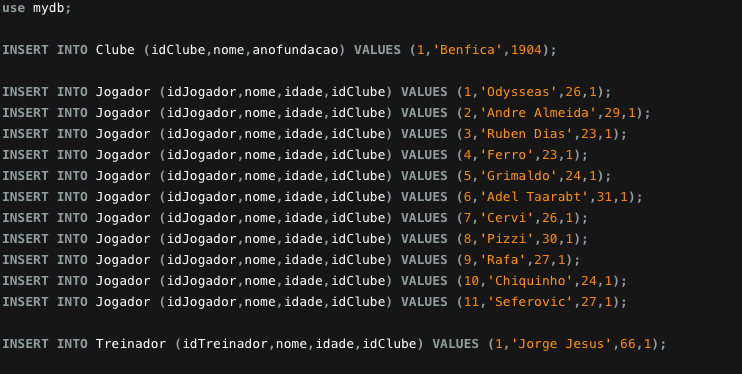
\includegraphics[width = 0.8\textwidth]{povoamento1.png}
  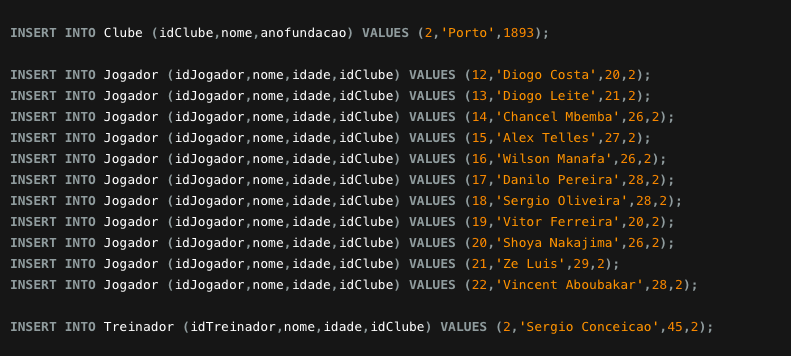
\includegraphics[width = 0.8\textwidth]{povoamento2.png}
  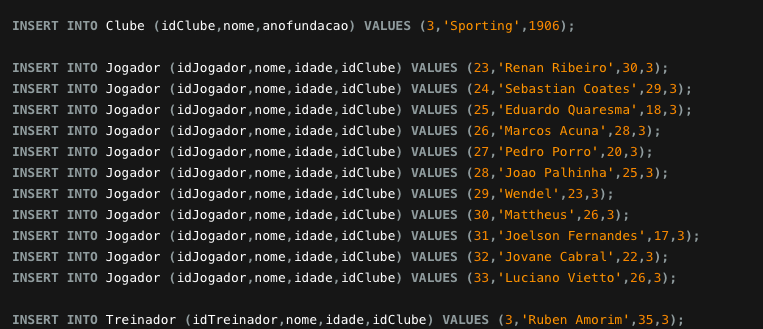
\includegraphics[width = 0.8\textwidth]{povoamento3.png}
  
  \caption {Script utilizado para realizar o povoamento da base de dados}

  \label{fig:povoamento}
\end{figure}


O povoamento da mesma pode ser confirmado realizando uma consulta á base de dados em questão como se mostra na figura abaixo:

\begin{figure}[H]

  \centering
  \captionsetup{justification=centering}

  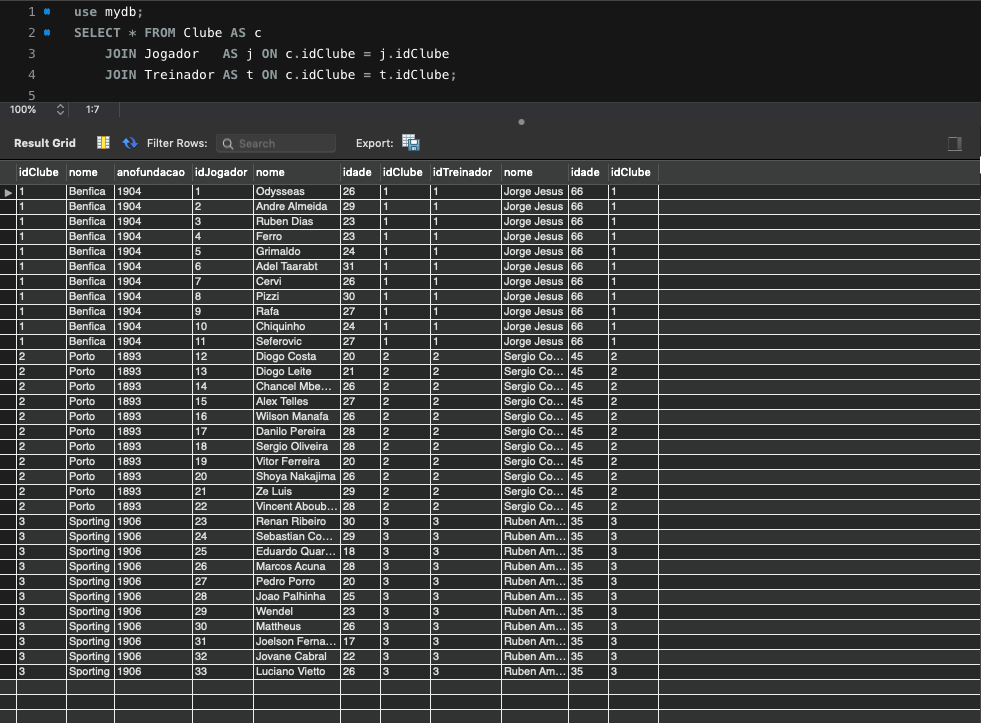
\includegraphics[width = 0.8\textwidth]{prova1.png}
  
  \caption {Visualização da base de dados povoada}

  \label{fig:baseDeDados}
\end{figure}

\newpage
\section{Questão 2}

Uma aplicação que permita ver equipas de futebol necessita de poder mostrar informações de um jogador especifico, informações de um treinador especifico, ou informações de uma equipa. Como se trata de uma base de dados doumental todas as informações associadas á equipa devem ser incluidas como documentos aninhados no documento da mesma, neste caso treinador e jogadores devem ser incluidos.
Assim a base de dados NoSQL MongoDB deverá ter 3 coleções, nomeadamente clube, jogador e treinador. Os documentos a produzir para cada coleção detalham-se em seguida com um exemplo:
\begin{enumerate}
	\item Clube
		\begin{figure}[H]

		  \centering
		  \captionsetup{justification=centering}

		  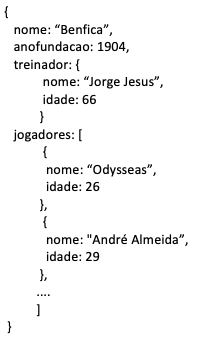
\includegraphics[scale = 0.5]{clube.png}
		  
		  \caption {Documento referente a um clube}
		\end{figure}
	\item Jogador
		\begin{figure}[H]

		  \centering
		  \captionsetup{justification=centering}

		  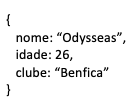
\includegraphics[scale = 0.5]{jogador.png}
		  
		  \caption {Documento referente a um jogador}
		\end{figure}
	\newpage
	\item Treinador
		\begin{figure}[H]

		  \centering
		  \captionsetup{justification=centering}

		  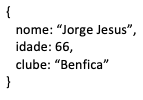
\includegraphics[scale = 0.5]{treinador.png}
		  
		  \caption {Documento referente a um treinador}
		\end{figure}
\end{enumerate}


\par Nota: Como para mim não é claro se devo ou não implementar a base de dados em MongoDB devido á questão 3 que se transcreve em seguida "Identifique as principais diferen\c{c}as da base de dados relacional acima descrita e a \textit{construida na alínea acima.}", decidi implementar a base de dados em Mongo para além de indicar a estrutura dos documentos.
\newline


\par Assim a base de dados foi criada e povoada recorrendo aos comandos listados no seguinte script. 

\begin{figure}[H]

  \centering
  \captionsetup{justification=centering}

  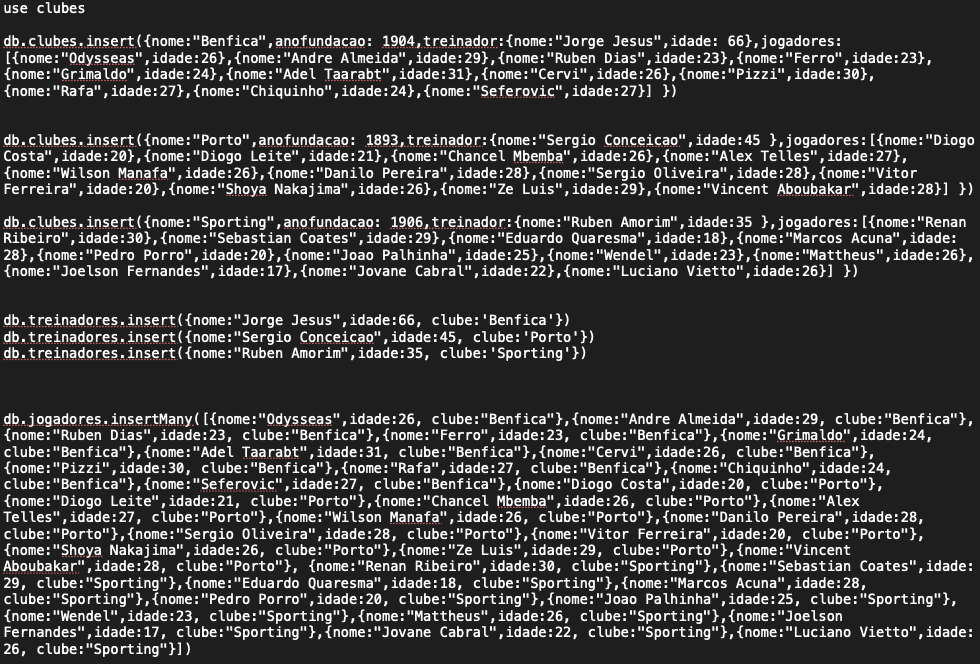
\includegraphics[width = \textwidth]{povoamentoMongo.png}
  
  \caption {Comandos usados para o povoamento da base de dados MongoDB}

  \label{fig:povoamento}
\end{figure}


\par A base de dados preenchida pode ser vista nas seguintes imagens.

\begin{figure}[H]

  \centering
  \captionsetup{justification=centering}

  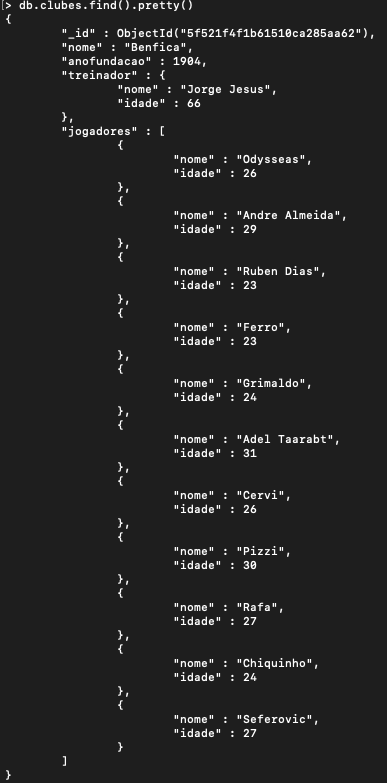
\includegraphics[width = 0.4\textwidth,height = 10cm]{clubes1.png}
  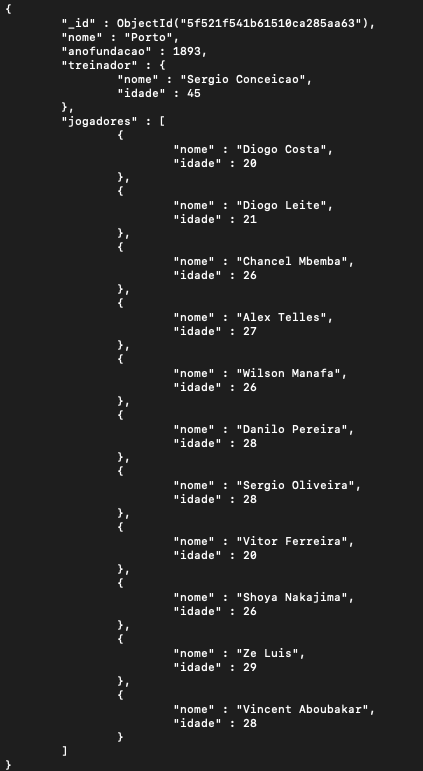
\includegraphics[width = 0.4\textwidth,height = 10cm]{clubes2.png}
  \caption {Documentos relativos aos clubes Benfica e Porto com a informação associada aninhada em subdocumentos}
  
  \vspace{0.5cm}
  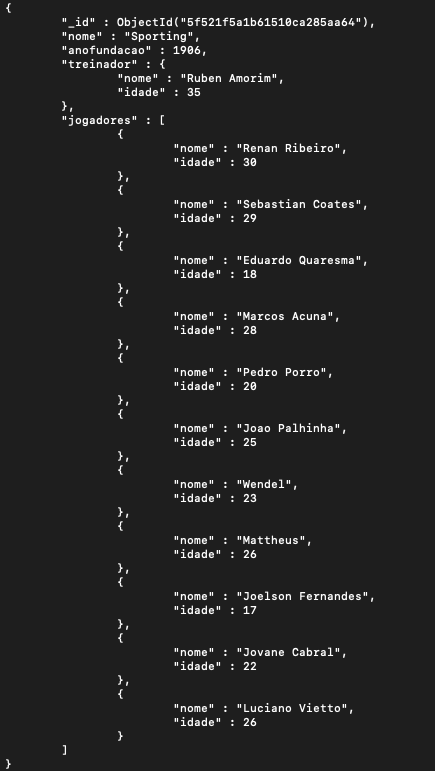
\includegraphics[width = 0.4\textwidth,height = 10cm]{clubes3.png}
  
  \caption {Documento relativo ao clube Sporting com a informação associada aninhada em subdocumentos}

  \label{fig:povoamento2}
\end{figure}

\begin{figure}[H]

  \centering
  \subfloat{{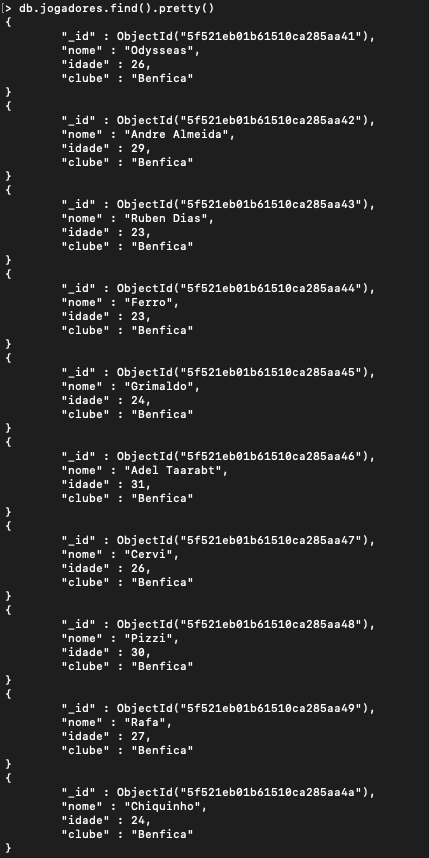
\includegraphics[width=.4\linewidth,height = 10cm]{jogadores1.png}}}
  \qquad
  \subfloat{{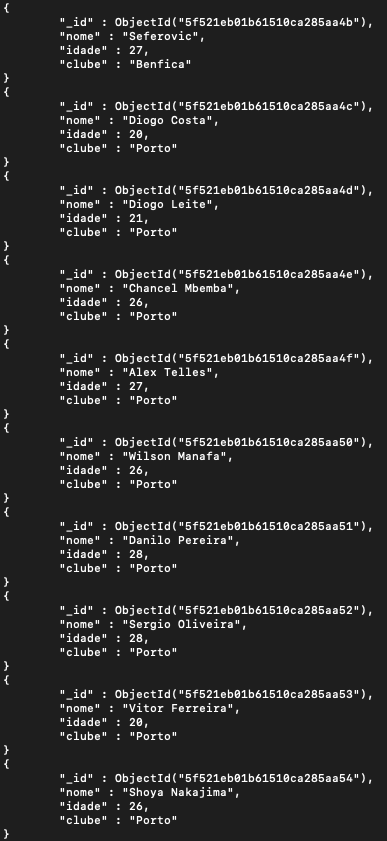
\includegraphics[width=.4\linewidth,height = 10cm]{jogadores2.png}}}
  \qquad
  \subfloat{{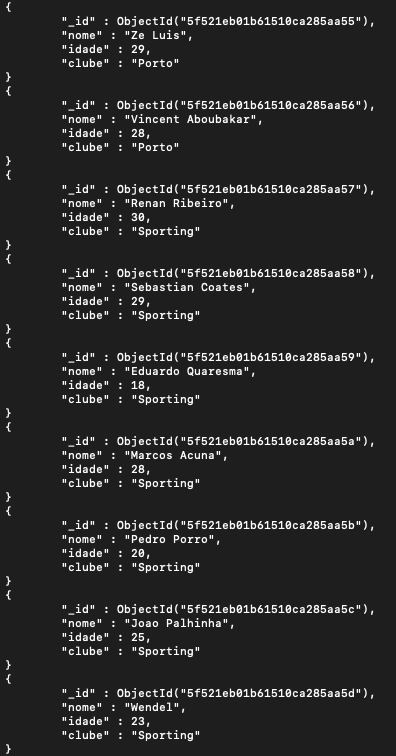
\includegraphics[width=.4\linewidth,height = 10cm]{jogadores3.png}}}
  \qquad
  \subfloat{{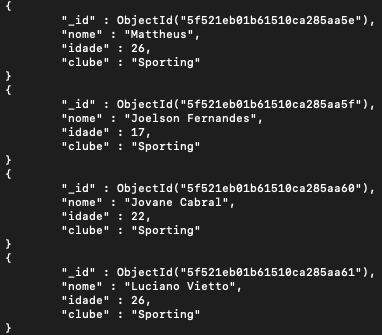
\includegraphics[width=.4\linewidth,height=5cm]{jogadores4.png}}}
  
  \caption {Documentos relativos aos jogadores}

  \label{fig:povoamento}
\end{figure}


\begin{figure}[H]

  \centering
  \captionsetup{justification=centering}

  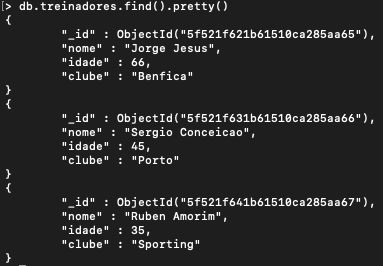
\includegraphics[width = 0.8\textwidth]{treinadores.png}
  
  \caption {Documentos relativos aos treinadores}

  \label{fig:povoamento}
\end{figure}










\newpage
\section{Questão 3}


As diferenças entre uma base de dados relacional e uma base de dados documental são as a seguir enunciadas:
\begin{itemize}
 \item Tabelas\hfill\newline
 \par Numa  base de dados relacional os dados referentes a uma entidade podem estar distribuidos por várias tabelas sendo que cada tabela contêm colunas que correspondem a atributos, linhas que correspondem cada uma a um registo e chaves estrangeiras e primárias para estabelecerem relações entre si. Já numa base de dados documental não se usam tabelas pra armazenar informação sobre uma entidade, em vez disso os dados relacionados como uma entidade são armazenados num único documento e todos os dados associados á mesma são aninhados dentro do mesmo.\hfill\newline
 \item Esquemas\hfill\newline
 \par Numa base de dados relacional antes de se inserir qualquer dado é criado um esquema lógico. Já nas bases de dados documentais podemos carregar os dados sem utilizarmos um esquema pré-definido.\hfill\newline
 \item Escalabilidade\hfill\newline
 \par Enquanto as bases de dados relacionais são adequadas a escalar verticalmente as bases de dados documentais podem ser dimensionadas horizontalmente (sharding) o que permite o armazenamento da base de dados em milhares de computadores sem comprometer o desempenho.\hfill\newline
 \item Relacionamentos\hfill\newline
 \par Como já foi referido anteriormente, os dados armazenados em tabelas nas bases de dados relacionais relacionam-se utilizando chaves estrangeiras. No entanto, nas bases de dados documentais não existem chaves estrangeiras, em vez disso os dados relacionados com uma entidade são aninhados dentro do documento da mesma.\hfill\newline
\item Linguagem \hfill\newline
 \par As bases de dados relacionais utilizam SQL como linguagem de interrogação da mesma. No MongoDB é utilizada uma sintaxe própria.
\end{itemize}

\newpage

%
% ---- Bibliography ----
%
% BibTeX users should specify bibliography style 'splncs04'.
% References will then be sorted and formatted in the correct style.
%
% \bibliographystyle{splncs04}
% \bibliography{mybibliography}
%
\begin{thebibliography}{8}

%\bibitem{ref_intro1}
%https://www.itu.int/en/ITU-D/Statistics/Pages/stat/default.aspx
\bibitem{ref_intro} https://www.mysql.com/products/workbench/

\end{thebibliography}
%\input{anexo.tex}

\end{document}